% Created 2017-05-18 四 21:51
\documentclass[11pt]{article}
\usepackage[utf8]{inputenc}
\usepackage[T1]{fontenc}
\usepackage{fixltx2e}
\usepackage{graphicx}
\usepackage{longtable}
\usepackage{float}
\usepackage{wrapfig}
\usepackage{rotating}
\usepackage[normalem]{ulem}
\usepackage{amsmath}
\usepackage{textcomp}
\usepackage{marvosym}
\usepackage{wasysym}
\usepackage{amssymb}
\usepackage{hyperref}
\tolerance=1000
\author{Qiu Wei, Lu Yizhou}
\date{\today}
\title{Assignment4 Report}
\hypersetup{
  pdfkeywords={},
  pdfsubject={},
  pdfcreator={Emacs 24.5.1 (Org mode 8.2.10)}}
\begin{document}

\maketitle
\tableofcontents


\section{Implementation}
\label{sec-1}
The code is seperated into two parts, \emph{kmeans.py} and \emph{main.py}.
\emph{main.py} parses the data and draw the graphs of different solution,
and \emph{kmeans.py} implemented the core function of k-means algorithm.

The k-means algorithm have the folloing steps:

\begin{itemize}
\item 1.Randomly choose k distinct points as centroids
\item 2.Partition the data points into k parts surrounding the k centroids
\item 3.Move the centroid of each parts to the arithmetic mean of the points in this part
\item 4.If the centroids converges, halt the algorithm. Otherwise repeat step 2,3
\end{itemize}

In each case, \emph{main.py} will run k-means algorithm for 100 times and record the
maximum, minimum and average diameters.
\section{Result and Analysis}
\label{sec-2}
The origin distribution is as following:

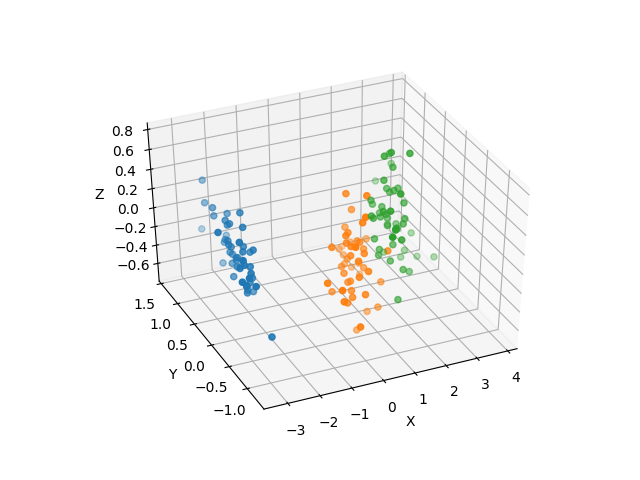
\includegraphics[width=.9\linewidth]{raw_data.png}

And we tried k=2,3,4 and calculated the maximum diameter of the k parts.

\begin{center}
\begin{tabular}{rrrr}
k & maximum diameter & minimum diameter & average diameter\\
2 & 6.91 & 3.91 & 4.72\\
3 & 4.86 & 2.58 & 3.07\\
4 & 4.70 & 2.41 & 2.52\\
\end{tabular}
\end{center}

Obviously, the diameter strictly decreases when k increase.
Now I will analyse each case in the following.

\subsection{k = 2}
\label{sec-2-1}
The distribution graph of the best result is as following:

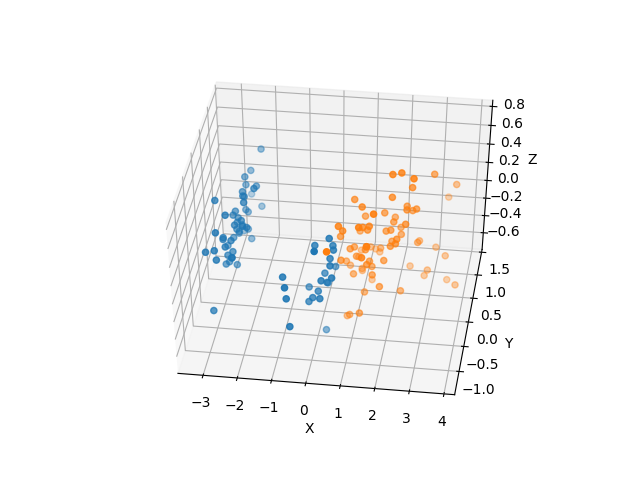
\includegraphics[width=.9\linewidth]{cluster=2.png}

This graphs show a problem of k-means algorithm:

In the middle of the picture some points was partitioned into wrong
class to reduce the maximum diameter.

Here is the question: the k-means algorithm can not tell a hollow sphere
and a dense sphere, so it will classify two distinct classes as one class.
Also this makes k-means algorithm sensitive with the original centroids.

\subsection{k = 3}
\label{sec-2-2}
The distribution graph of the best result is as following:

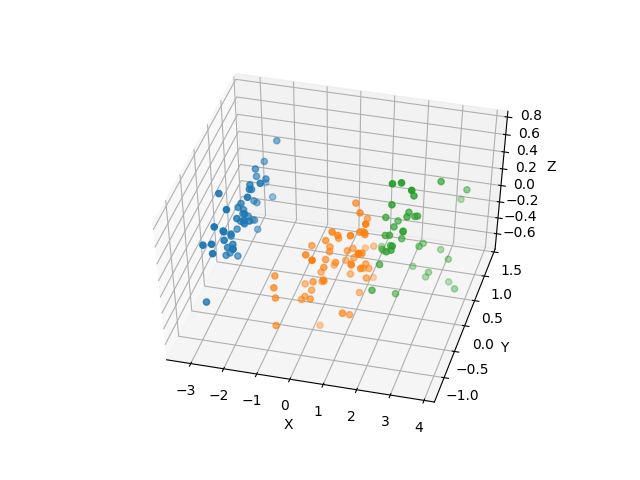
\includegraphics[width=.9\linewidth]{cluster=3.png}

Obviously this distribution is similar with the original graph.

\subsection{k = 4}
\label{sec-2-3}
The distribution graph of the best result is as following:

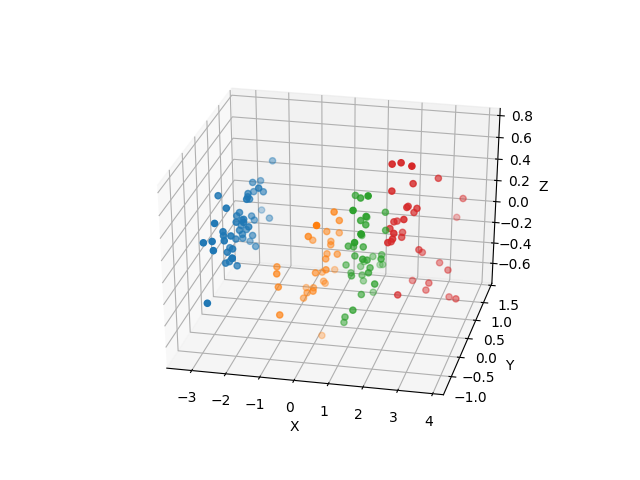
\includegraphics[width=.9\linewidth]{cluster=4.png}

This distribution is just seperate two class in original distribution into
three class. And it do not benefit a lot to the diameter.
% Emacs 24.5.1 (Org mode 8.2.10)
\end{document}